\documentclass{beamer}
\usepackage[utf8]{inputenc}
\usepackage[german]{babel}
\usepackage{graphicx}
\usepackage{tikz}
\usepackage[autostyle=true,german=quotes]{csquotes}
\MakeOuterQuote{"}
\begin{document}

\addtobeamertemplate{navigation symbols}{}{%
    \usebeamerfont{footline}%
    \usebeamercolor[fg]{footline}%
    \hspace{1em}%
    \insertframenumber/\inserttotalframenumber
}
\setbeamertemplate{navigation symbols}{}
\usebackgroundtemplate{
  \tikz\node[opacity=0.3]
  {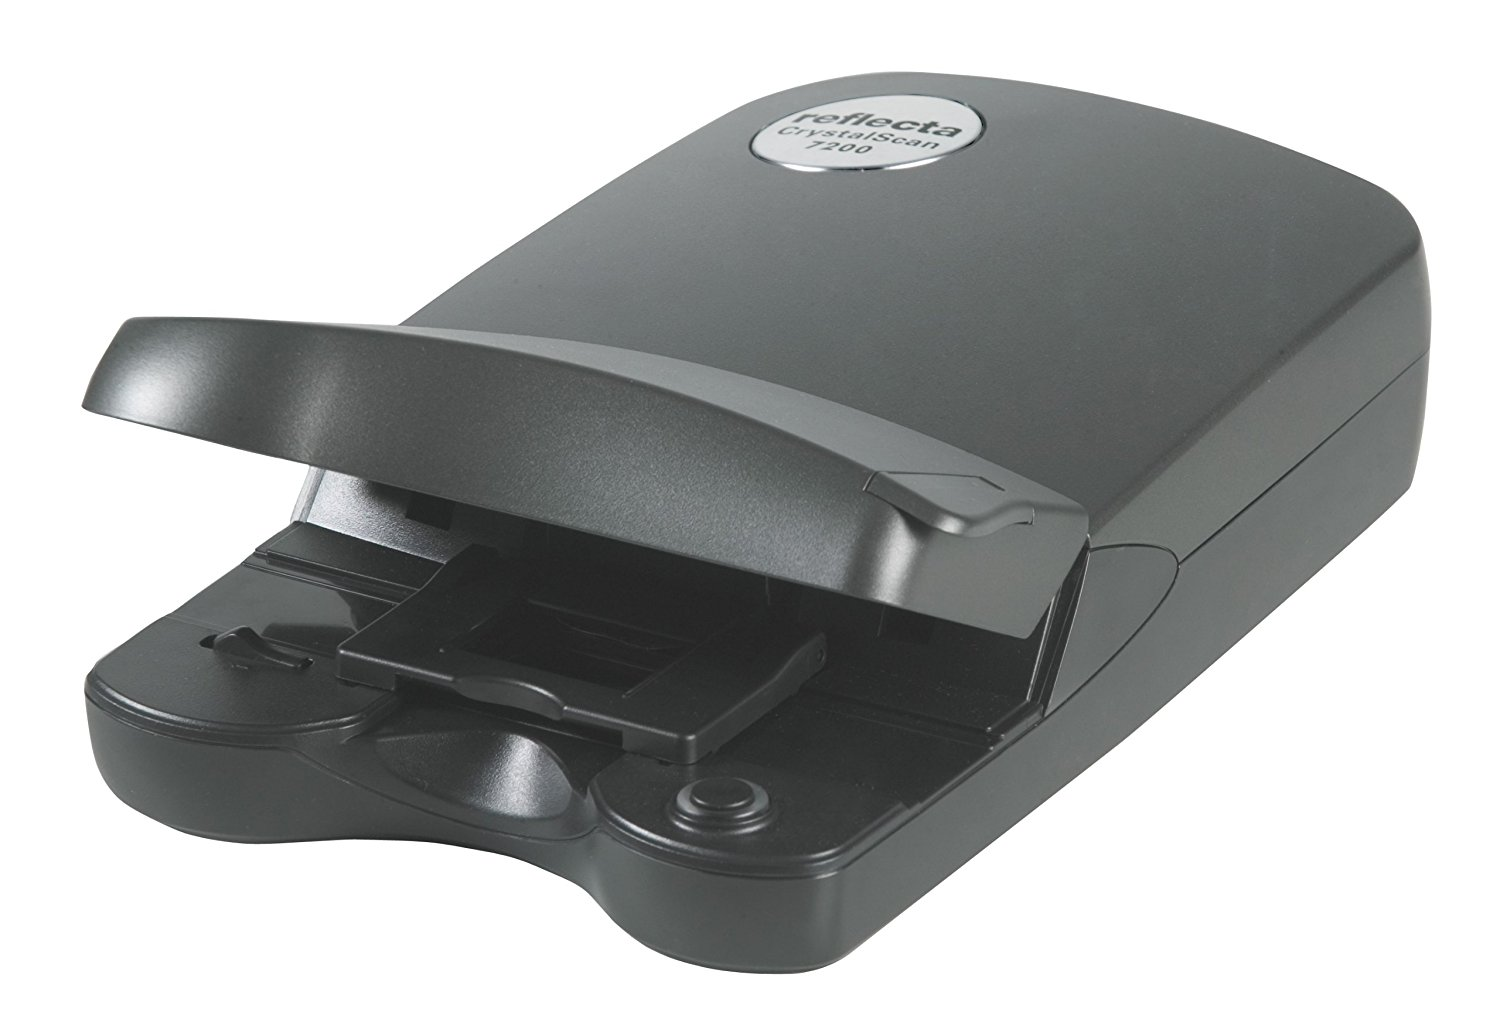
\includegraphics[height=\paperheight,width=\paperwidth]
  {images/presentation/the_scanner.jpg}};
}
\title{Entwicklung eines Treibers für einen Filmscanner mittels USB-Sniffing und Reverse Engineering}
\author{Hugo Platzer}
\date{}

\frame{\titlepage}

\usebackgroundtemplate{}
\frame{\frametitle{Reflecta CrystalScan 7200}
  \begin{itemize}
    \item Für Kleinbilddias / -negative
    \item Per USB verbunden
    \item Software nur für Windows / Mac
    \item Versuch, einen Linux-Treiber zu entwickeln ohne entsprechende
          Dokumentation
  \end{itemize}
}

\frame{\frametitle{Reverse Engineering}
  \begin{itemize}
    \item Prozess des "Engineering" (von der Spezifikation zum Produkt) in
          umgekehrter Richtung
    \item Versuch, aus für den Konsumenten verfügbaren Daten (Maschinencode,
          Mitlauschen an Schnittstellen) Protokolle rekonstruieren
    \item Rechtliche Grauzone
    \item Um Einverständnis gebeten: Hersteller war kooperativ
  \end{itemize}
}

\frame{\frametitle{Der USB-Standard}
  \begin{itemize}
    \item ein Anschluss für alle Klassen von Geräten
    \item Alle Kommunikation geht vom Host aus
    \item Verschiedene Übertragungsmodi (Control, Bulk, Interrupt, Isochronous)
  \end{itemize}
}

\frame{\frametitle{USB-Sniffing}
  \begin{itemize}
    \item Mitschneiden der Kommunikation zwischen Gerät und Windows-Software
    \item Kernelmodul {\tt usbmon}
    \begin{itemize}
      \item Zugang zu vom Linux-Kernel abgearbeiteten USB-Transfers
      \item Schwierigkeiten bei langer Payload
    \end{itemize}
    \item Wireshark
    \begin{itemize}
      \item Netzwerk-Sniffer, der sich auch für USB eignet
      \item sowohl zur Aufzeichnung als auch Analyse
      \item Deaktivierung aller Protokolle außer USB
    \end{itemize}
    \item VirtualBox
    \begin{itemize}
      \item Windows in virtueller Maschine unter Linux ausführen
      \item USB-Passthrough gibt Windows Zugang zum Scanner
    \end{itemize}
  \end{itemize}
}

\frame{\frametitle{usbmon: unvollständige Payload}
  \begin{itemize}
    \item Bei großen Paketen wird Payload nach 60KB abgeschnitten
    \item visuell: Risse im rekonstruierten Bild
    \item gelöst durch einfachen Kernel-Patch
  \end{itemize}
}


\frame{\frametitle{Analyse der Aufzeichnung}
  \begin{itemize}
    \item Versuche, Bilddaten aus Aufzeichnung zu rekonstruieren
    \item Beispiel: Rohdaten der Bulk-Transfers: Schließen auf Little-Endian 16bit Pixelwerte
    \item Ermitteln von: Offset, Zeilenlänge, Farbkanäle (Interleaving), Offsets
  \end{itemize}
}

\frame{\frametitle{Ansteuern des Scanners}
  \begin{itemize}
    \item Grundidee: aufgezeichnete Befehle zum Gerät wieder abspielen, eingehende Daten speichern
    \item Kommunikation läuft nach gewissen Mustern ab
    \item Warten auch wichtig: Zeitdiagramm
    \item Welche Bytes haben welche Funktion?
    \begin{itemize}
      \item Wiederhole Scan mit jeweils einem geänderten Parameter
      \item Beispiel: Auflösung, Farbmodus, Scanbereich
    \end{itemize}
  \end{itemize}
}

\frame{\frametitle{Bildverarbeitung}
  \begin{itemize}
    \item Helligkeitsunterschiede pro Spalte ausgleichen
    \item Gammakorrektur, Wertebereich, Farbbalance
    \item Staub- / Kratzerkorrektur (Digital ICE, Inpainting)
    \item automatisches Zuschneiden
    
  \end{itemize}
}

\frame{\frametitle{Ausblick: SANE}
  \begin{itemize}
    \item Das Linux-Scannerframework
    \item hat Treiber für CrystalScan 7200, funktioniert aber nicht
    \item meine Software in SANE integrieren
  \end{itemize}
}

\begin{frame}[plain,c]
\usebeamerfont*{frametitle}\usebeamercolor[fg]{frametitle}

\begin{center}
Live-Demo
\end{center}

\end{frame}
\end{document}
